%===============================================================================
% SYNDICATION Developer Guide
%===============================================================================
% $Id: developer-guide.tex 257 2005-01-31 10:52:20Z thom $
%===============================================================================


%===============================================================================
% Configuration
%===============================================================================


%-------------------------------------------------------------------------------
% \documentclass and \usepackage directives
%-------------------------------------------------------------------------------
\documentclass[a4paper,fleqn]{report}
%\usepackage{ngerman}
\usepackage[latin1]{inputenc}
\usepackage[T1]{fontenc}
\usepackage[small,hang,bf]{caption2}
\usepackage{fancyhdr}
\usepackage[nice]{nicefrac}
\usepackage{color,listings}
\usepackage{alltt}


% Compilation with latex or pdflatex?
\newif\ifpdf 
\ifx\pdfoutput\undefined 
  \pdffalse
\else
  \pdfoutput=1 
  \pdftrue 
\fi 

% Compilation with pdflatex
\ifpdf
 
  \usepackage[pdftex]{graphicx}

  \usepackage[
    pdftex,
    a4paper,
    bookmarks,
    pdfstartview=FitH,    % starts with page width
    bookmarksopen,        % opens index
    bookmarksnumbered,    % index with numbering
    colorlinks,           % links with color, otherwise with border
    linkcolor=blue,       % Standard red
    citecolor=blue,       % Standard green
    urlcolor=magenta,     % Standard cyan
    filecolor=blue
  ]{hyperref} 

  \pdfinfo{
    /Title      (EiffelRSS SYNDICATION Developer Guide)
    /Author     (Thomas Weibel, Martin Luder, Michael K�ser)
    /Subject    (Eiffel programming)
    /Keywords   (Programming, EiffelRSS)
  }

  % Use default Acrobat reader fonts
  \usepackage{mathpazo}

  % Use CM fonts (increases document size)
  % \usepackage{ae}

% Compilation with latex
\else 

  \usepackage{graphicx} 

\fi


%-------------------------------------------------------------------------------
% Configure \maketitle
%-------------------------------------------------------------------------------
\title{EiffelRSS \\ SYNDICATION \\ Developer Guide}
\author{
  Michael K\"aser <kaeserm@student.ethz.ch>
  \and 
  Martin Luder <luderm@student.ethz.ch>
  \and 
  Thomas Weibel <weibelt@student.ethz.ch>
}
\date{\today}


%-------------------------------------------------------------------------------
% Configure fancyhdr
%-------------------------------------------------------------------------------
\pagestyle{fancy}

\renewcommand{\headrulewidth}{0.1 pt}
\renewcommand{\footrulewidth}{0.1 pt}

\fancypagestyle{plain}{
  \lhead{\nouppercase{\leftmark}}
  \chead{}
  \rhead{\thepage}
  \lfoot{EiffelRSS}
  \cfoot{}
  \rfoot{SYNDICATION Developer Guide}
}

\lhead{\nouppercase{\leftmark}}
\chead{}
\rhead{\thepage}

\lfoot{EiffelRSS}
\cfoot{}
\rfoot{SYNDICATION Developer Guide}


%-------------------------------------------------------------------------------
% Configure listings
%-------------------------------------------------------------------------------
\lstset{showstringspaces=false,
  breaklines=true,
  breakindent=0pt,
  prebreak=\mbox{\tiny$\searrow$},
  postbreak=\mbox{{\color{blue}\tiny$\rightarrow$}},
  frame=trBL,
  framerule=0.75pt,
  framesep=4pt,
  rulesep=0.75pt  
}


%-------------------------------------------------------------------------------
% Common configuration
%-------------------------------------------------------------------------------
\setlength{\parindent}{0em}
\setlength{\parskip}{1.5ex plus0.5ex minus0.5ex}
\sloppy
\setlength{\mathindent}{0em}


%-------------------------------------------------------------------------------
% Commandos
%-------------------------------------------------------------------------------
\newcommand{\hr}{\rule{\textwidth}{1pt}}


%===============================================================================
% Document
%===============================================================================
\begin{document}

\begin{titlepage}
  \newlength{\centeroffset}
  \setlength{\centeroffset}{-0.5\oddsidemargin}
  \addtolength{\centeroffset}{0.5\evensidemargin}

  \thispagestyle{empty}

  \noindent
\includegraphics[width=\textwidth]{../../figures/big_ETH}\\[-3mm]
  \hr

  \vspace*{\stretch{1}}

  \makebox[0pt][l]{
    \begin{minipage}{\textwidth}
      \flushright{
        \Huge\bfseries EiffelRSS
      }

      \noindent\rule{\textwidth}{3pt}\\[2.5ex]

      \hfill\emph{
        \Large SYNDICATION Developer Guide
      }
    \end{minipage}
  }

  \vspace{\stretch{1}}

  \makebox[0pt][l]{
    \begin{minipage}{\textwidth}
      \flushright{
        \bfseries 
        Michael K\"aser <kaeserm@student.ethz.ch>\\[0.3ex]
        Martin Luder <luderm@student.ethz.ch>\\[0.3ex]
        Thomas Weibel <weibelt@student.ethz.ch>\\[0.3ex]
      }
    \end{minipage}
  }

  \vspace{\stretch{1}}

  \noindent\hr\\[1mm]
  
\includegraphics[width=\textwidth]{../../figures/big_inf}
\end{titlepage}

% Use roman page numbering
\pagenumbering{roman}

\begin{abstract}
  \texttt{SYNDICATION} is the main cluster of EiffelRSS with a feed
  object model and classes to load / write feeds. It is divided into
  three subclusters.
\end{abstract}

\clearpage
\tableofcontents

\clearpage
\listoffigures

\newpage

% Set page counter to zero
\setcounter{page}{0} 

% Use arabic page numbering
\pagenumbering{arabic}


%-------------------------------------------------------------------------------
% Part: INTERFACE
%-------------------------------------------------------------------------------
%-------------------------------------------------------------------------------
% Part: INTERFACE
%-------------------------------------------------------------------------------
\part{INTERFACE}


%-------------------------------------------------------------------------------
% Chapter: Overview
%-------------------------------------------------------------------------------
\chapter{Overview}
\label{cha:overview}

\texttt{INTERFACE} is the sub-cluster of syndication with all the
classes a developer needs to use the library. There are classes to
read into and write from a \texttt{FEED}, a \texttt{FEED\_MANAGER} to
administrate a list of \texttt{FEED}s, and a factory class which makes
it easy to create all necessary objects.

See figure \ref{fig:interface} for an overview of the cluster.

\begin{figure}[htbp]
  \centering
  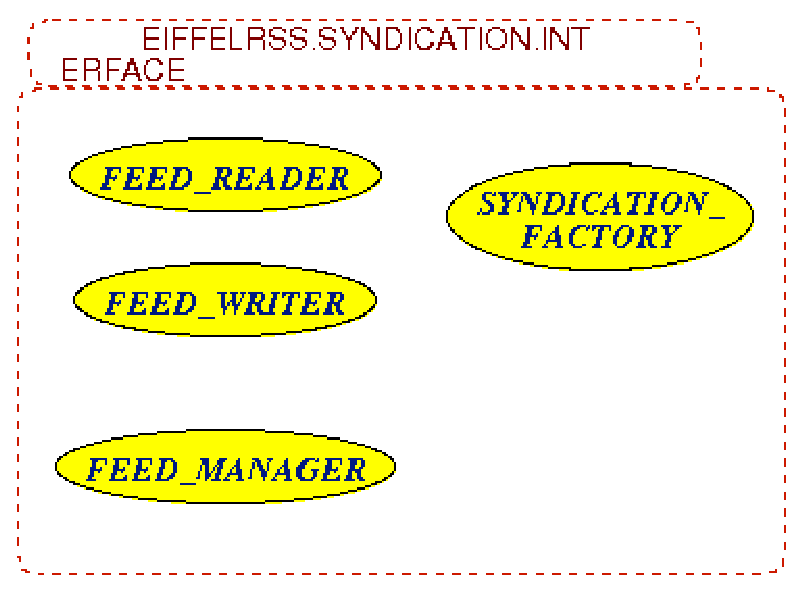
\includegraphics[scale=.6]{./figures/EIFFELRSS_SYNDICATION_INTERFACE}
  \caption{BON diagram of cluster \texttt{INTERFACE}}
  \label{fig:interface}
\end{figure}


%-------------------------------------------------------------------------------
% Chapter: Class SYNDICATION_FACTORY
%-------------------------------------------------------------------------------
\chapter{Class SYNDICATION\_FACTORY}
\label{cha:syndiction-factory}


\section{Overview}
\label{sec:syndication-factory-overview}

\texttt{SYNDICATION\_FACTORY} provides an easy way to create objects
of classes from the cluster \texttt{SYNDICATION}.


\section{Usage}
\label{sec:syndication-factory-usage}

\begin{lstlisting}[language=Eiffel]
class USAGE_EXAMPLE

create 
  make

feature -- Initialization

  make is
      -- Creation procedure.
    do      
      create syndication

      feed := syndication.new_feed ("EiffelRSS", create {HTTP_URL}.make ("http://eiffelrss.berlios.de/"), "EiffelRSS news")

      item := syndication.new_item (channel, "Version 23 released!", create {HTTP_URL}.make ("http://eiffelrss.berlios.de/Main/News"), "Version 23 of EiffelRSS got release today. Happy syndicating!")

      feed.add_item (item)
    end
    
feature -- Arguments

  syndication: SYNDICATION_FACTORY
      -- Syndication factory object

  feed: FEED
      -- Feed object
      
  item: ITEM
      -- Item object
  
end -- class USAGE_EXAMPLE
\end{lstlisting}


\section{Features}
\label{sec:syndication-factory-features}


\subsection{READER factory}
\label{sec:syndication-factory-reader}

\subsubsection{new\_reader\_from\_url }

\begin{lstlisting}[language=Eiffel]
new_reader_from_url (a_url: STRING): FEED_READER
  -- Create with `a_url' as source of feed
\end{lstlisting}


\subsection{WRITER factory}
\label{sec:syndication-factory-writer}

\subsubsection{new\_writer\_from\_feed}

\begin{lstlisting}[language=Eiffel]
new_writer_from_feed (a_feed: FEED): FEED_WRITER
  -- Create a writer object for the feed `a_feed'
\end{lstlisting}


\subsection{FEED\_MANAGER factory}
\label{sec:syndication-factory-feed-manager}

\subsubsection{new\_feed\_manager}

\begin{lstlisting}[language=Eiffel]
new_feed_manager: FEED_MANAGER
  -- Create a new feed manager with default refresh period `30'
\end{lstlisting}


\subsubsection{new\_feed\_manager\_custom}

\begin{lstlisting}[language=Eiffel]
new_feed_manager_custom (a_refresh_period: INTEGER): FEED_MANAGER
  -- Create a new feed manager with default refresh period `a_refresh_period'
\end{lstlisting}


\subsection{FEED factory}
\label{sec:syndication-factory-feed}

\subsubsection{new\_feed}

\begin{lstlisting}[language=Eiffel]
new_feed (a_title: STRING; a_link: URL; a_description: STRING): FEED
  --  Create a feed with title, link and description
\end{lstlisting}


\subsubsection{new\_feed\_from\_channel}

\begin{lstlisting}[language=Eiffel]
new_feed_from_channel (a_channel: CHANNEL): FEED
  -- Create a new feed from an existing channel
\end{lstlisting}


\subsection{CHANNEL factory}
\label{sec:syndication-factory-channel}

\subsubsection{new\_channel}

\begin{lstlisting}[language=Eiffel]
new_channel (a_title: STRING; a_link: URL; a_description: STRING): CHANNEL
  --  Create a channel with title, link and description
\end{lstlisting}


\subsubsection{new\_channel\_cloud}

\begin{lstlisting}[language=Eiffel]
new_channel_cloud (a_domain: STRING; a_port: INTEGER; a_path: STRING; a_register_procedure: STRING; a_protocol: STRING): CHANNEL_CLOUD
  -- Create a channel cloud with domain, port, path, register procedure and protocol
\end{lstlisting}


\subsubsection{new\_channel\_image}

\begin{lstlisting}[language=Eiffel]
new_channel_image (a_url: URL; a_title: STRING; a_link: URL): CHANNEL_IMAGE
  -- Create a channel image with URL, title, and link
\end{lstlisting}


\subsubsection{new\_channel\_text\_input}

\begin{lstlisting}[language=Eiffel]
new_channel_text_input (a_title: STRING; a_description: STRING; a_name: STRING; a_link: URL): CHANNEL_TEXT_INPUT
  -- Create a channel text input with title, description, name and link
\end{lstlisting}


\subsection{ITEM factory}
\label{sec:syndication-factory-item}

\subsubsection{new\_item}

\begin{lstlisting}[language=Eiffel]
new_item (a_channel: CHANNEL; a_title: STRING; a_link: URL; a_description: STRING): ITEM
  -- Create an item with title, link and description
\end{lstlisting}


\subsubsection{new\_item\_with\_title}

\begin{lstlisting}[language=Eiffel]
new_item_with_title (a_channel: CHANNEL; a_title: STRING): ITEM
  -- Create an item with title
\end{lstlisting}


\subsubsection{new\_item\_with\_description}

\begin{lstlisting}[language=Eiffel]
new_item_with_description (a_channel: CHANNEL; a_description: STRING): ITEM
  -- Create an item with description
\end{lstlisting}


\subsubsection{new\_item\_enclosure}

\begin{lstlisting}[language=Eiffel]
new_item_enclosure (a_url: URL; a_length: INTEGER; a_type: STRING): ITEM_ENCLOSURE
  -- Create an item enclosure
\end{lstlisting}


\subsubsection{new\_item\_guid}

\begin{lstlisting}[language=Eiffel]
new_item_guid (a_guid: STRING): ITEM_GUID
  -- Create an item guid with `is_perma_link' set to False
\end{lstlisting}


\subsubsection{new\_item\_guid\_perma\_link}

\begin{lstlisting}[language=Eiffel]
new_item_guid_perma_link (a_guid: STRING): ITEM_GUID
  -- Create an item guid with `is_perma_link' set to True
\end{lstlisting}


\subsubsection{new\_item\_source}

\begin{lstlisting}[language=Eiffel]
new_item_source (a_name: STRING; a_url: URL): ITEM_SOURCE
  -- Create an item source
\end{lstlisting}


\subsection{CATEGORY factory}
\label{sec:syndication-factory-category}

\subsubsection{new\_category}

\begin{lstlisting}[language=Eiffel]
new_category: CATEGORY
  -- Create a category with title `[unnamed category]')
\end{lstlisting}


\subsubsection{new\_category\_with\_title}

\begin{lstlisting}[language=Eiffel]
new_category_with_title (a_title: STRING): CATEGORY
  -- Create a category with title `a_title'
\end{lstlisting}


\subsubsection{new\_category\_with\_title\_domain}

\begin{lstlisting}[language=Eiffel]
new_category_with_title_domain (a_title: STRING; a_domain: URL): CATEGORY
  -- Create a category with title `a_title' and domain `a_domain'
\end{lstlisting}


%-------------------------------------------------------------------------------
% Chapter: Class FEED_MANAGER
%-------------------------------------------------------------------------------
\chapter{Class FEED\_MANAGER}
\label{cha:feed-manager}

\section{Overview}
\label{sec:feed-manager-overview}

\texttt{FEED\_MANAGER} is a class to manage feeds. It provides
features to add, remove and refresh feeds.

See figure \ref{fig:feed-manager} for an overview of the class.

\begin{figure}[htbp]
  \centering
  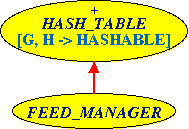
\includegraphics[scale=.6]{./figures/FEED_MANAGER}
  \caption{BON diagram of class \texttt{FEED\_MANAGER}}
  \label{fig:feed-manager}
\end{figure}


\section{Usage}
\label{sec:feed-manager-usage}

\begin{lstlisting}[language=Eiffel]
class
  FEED_MANAGER_EXAMPLE

create
  make

feature -- Initialization

  make is
      -- Creation procedure.
    do
      -- Create a simple feed
      create feed.make ("EiffelRSS", create {HTTP_URL}.make ("http://eiffelrss.berlios.de"), "EiffelRSS news")
      feed.set_refresh_period (15)
      feed.set_last_updated (create {DATE_TIME}.make_now)
      
      -- Add some simple items, use `feed.last_added_item' or directly create an item for finer control
      feed.new_item ("Version 23 released!", create {HTTP_URL}.make ("http://eiffelrss.berlios.de/Main/News"), "Version 23 of EiffelRSS got release today. Happy syndicating!")

      feed.new_item ("EiffelRSS wins award", create {HTTP_URL}.make ("http://eiffelrss.berlios.de/Main/Awards"), "EiffelRSS has been awarded by ISE as best syndication software written in Eiffel. For more info see award-winning pages: http://eiffelrss.berlios.de")

      -- Create feed manager
      create feed_manager.make
      feed_manager.add (feed, "http://eiffelrss.berlios.de/Main/AllRecentChanges?action=rss")
      feed_manager.refresh_all
    end
    
feature -- Arguments

  feed: FEED
      -- Example feed
      
  feed_manager: FEED_MANAGER
      -- Feed manager

end -- class FEED_MANAGER_EXAMPLE
\end{lstlisting}

\newpage

\section{Features}
\label{sec:feed-manager-features}

\subsection{Initialization}
\label{sec:feed-manager-initialization}

\subsubsection{make}

\begin{lstlisting}[language=Eiffel]
make
    -- Create a new feed manager with default refresh period `30'

\end{lstlisting}


\subsubsection{make\_custom}

\begin{lstlisting}[language=Eiffel]
make_custom (a_refresh_period: INTEGER)
    -- Create a new feed manager with default refresh period `a_refresh_period'
\end{lstlisting}


\subsection{Access}
\label{sec:feed-manager-access}

\subsubsection{default\_refresh\_period}

\begin{lstlisting}[language=Eiffel]
default_refresh_period: INTEGER
    -- Default refresh period in minutes
\end{lstlisting}

\subsubsection{last\_added\_feed}

\begin{lstlisting}[language=Eiffel]
last_added_feed: FEED
    -- feed that was last added
\end{lstlisting}

\subsubsection{feed\_addresses}

\begin{lstlisting}[language=Eiffel]
feed_addresses: LINKED_LIST[STRING]
    -- Returns a sortable list representation of the feeds saved in FEED_MANAGER
\end{lstlisting}

\subsubsection{feed\_links}

\begin{lstlisting}[language=Eiffel]
feed_links: LINKED_LIST[STRING]
    -- Returns a sortable list representation of the feeds saved in FEED_MANAGER
\end{lstlisting}


\subsection{Setter}
\label{sec:feed-manager-setter}

\subsubsection{set\_default\_refresh\_period}

\begin{lstlisting}[language=Eiffel]
set_default_refresh_period (a_refresh_period: INTEGER)
    -- Set refresh periode in minutes
\end{lstlisting}


\subsection{Element change}
\label{sec:feed-manager-element-change}

\subsubsection{add}

\begin{lstlisting}[language=Eiffel]
add (feed: FEED; url: STRING)
    -- Add `feed'
\end{lstlisting}

\subsubsection{add\_from\_url}

\begin{lstlisting}[language=Eiffel]
add_from_url (url: STRING)
    -- Add feed with URL `url'
\end{lstlisting}


\subsection{Refresh}
\label{sec:feed-manager-refresh}

\subsubsection{refresh}

\begin{lstlisting}[language=Eiffel]
refresh (url: STRING)
    -- Refresh feed with URL `url', if the feed is outdated
\end{lstlisting}

\subsubsection{refresh\_force}

\begin{lstlisting}[language=Eiffel]
refresh_force (url: STRING)
    -- Refresh feed with URL `url', even if the feed is not outdated
\end{lstlisting}

\subsubsection{refresh\_all}

\begin{lstlisting}[language=Eiffel]
refresh_all
    -- Refresh all feeds, if they are outdated
\end{lstlisting}

\subsubsection{refresh\_all\_force}

\begin{lstlisting}[language=Eiffel]
refresh_all_force
    -- Refresh all feeds, even if they are not outdated
\end{lstlisting}


\subsection{Conversion}
\label{sec:feed-manager-conversion}

\subsubsection{list\_representation}

\begin{lstlisting}[language=Eiffel]
list_representation: SORTABLE_TWO_WAY_LIST[FEED]
    -- Returns a sortable list representation of the feeds saved in FEED_MANAGER
\end{lstlisting}


\subsection{Conversion (sort)}
\label{sec:feed-manager-conversion-sort}

\subsubsection{sorted\_by\_last\_updated}

\begin{lstlisting}[language=Eiffel]
sorted_by_last_updated: SORTABLE_TWO_WAY_LIST[FEED]
    -- Returns a sorted list representation of the feeds, sorted by `last_updated'
\end{lstlisting}

\subsubsection{sorted\_by\_title}

\begin{lstlisting}[language=Eiffel]
sorted_by_title: SORTABLE_TWO_WAY_LIST[FEED]
    -- Returns a sorted list representation of the feeds, sorted by `title'
\end{lstlisting}

\subsubsection{sorted\_by\_link}

\begin{lstlisting}[language=Eiffel]
sorted_by_link: SORTABLE_TWO_WAY_LIST[FEED]
    -- Returns a sorted list representation of the feeds, sorted by `link'
\end{lstlisting}

\subsubsection{sorted\_by\_description}

\begin{lstlisting}[language=Eiffel]
sorted_by_description: SORTABLE_TWO_WAY_LIST[FEED]
    -- Returns a sorted list representation of the feeds, sorted by `description'
\end{lstlisting}

\subsubsection{reverse\_sorted\_by\_last\_updated}

\begin{lstlisting}[language=Eiffel]
reverse_sorted_by_last_updated: SORTABLE_TWO_WAY_LIST[FEED]
    -- Returns a sorted list representation of the feeds, reverse sorted by `last_updated'
\end{lstlisting}

\subsubsection{reverse\_sorted\_by\_title}

\begin{lstlisting}[language=Eiffel]
reverse_sorted_by_title: SORTABLE_TWO_WAY_LIST[FEED]
    -- Returns a sorted list representation of the feeds, reverse sorted by `title'
\end{lstlisting}

\subsubsection{reverse\_sorted\_by\_link}

\begin{lstlisting}[language=Eiffel]
reverse_sorted_by_link: SORTABLE_TWO_WAY_LIST[FEED]
    -- Returns a sorted list representation of the feeds, reverse sorted by `link'
\end{lstlisting}

\subsubsection{reverse\_sorted\_by\_description}

\begin{lstlisting}[language=Eiffel]
reverse_sorted_by_description: SORTABLE_TWO_WAY_LIST[FEED]
    -- Returns a sorted list representation of the feeds, reverse sorted by `description'
\end{lstlisting}


%-------------------------------------------------------------------------------
% Chapter: Class FEED_READER
%-------------------------------------------------------------------------------
\chapter{Class FEED\_READER}
\label{cha:feed-reader}

\section{Overview}
\label{sec:feed-reader-overview}

\texttt{FEED\_READER} is a helper class which manages everything to
load a feed.  It converts the data to an XML document object, detects
the format of the feed and uses the according reader object to convert
the XML document into a \texttt{FEED} object.

See figure \ref{fig:feed-reader} for an overview of the class.

\begin{figure}[htbp]
  \centering
  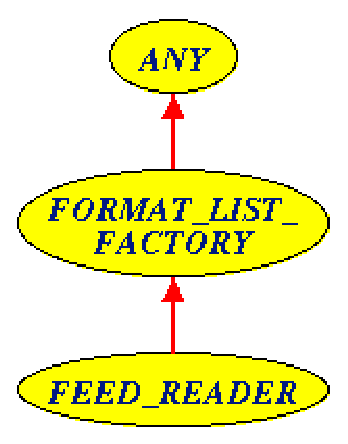
\includegraphics[scale=.6]{./figures/FEED_READER}
  \caption{BON diagram of class \texttt{FEED\_READER}}
  \label{fig:feed-reader}
\end{figure}


\section{Usage}
\label{sec:feed-reader-usage}

\begin{lstlisting}[language=Eiffel]
class
  READER_EXAMPLE

create
  make

feature -- Initialization

  make is
      -- Creation procedure.
    local
      location: STRING
      reader: FEED_READER
      feed: FEED
    do
      -- Get a feed location from the user
      io.put_string ("Enter an URL: ")
      io.read_line
      
      location := io.last_string.twin
      
      -- Create the reader
      create reader.make_url (location)
      
      -- Get the feed
      feed := reader.read
      
      -- Print feed
      io.put_string ("%NReceived feed:%N")
      io.put_string ("==============%N%N%N")
      io.put_string (feed.to_string)
    end

end -- class READER_EXAMPLE
\end{lstlisting}


\section{Features}
\label{sec:feed-reader-features}

\subsection{Initialization}
\label{sec:feed-reader-initialization}

\subsubsection{make\_url}

\begin{lstlisting}[language=Eiffel]
make_url (a_url: STRING)
  -- Create with `a_url' as source of feed
\end{lstlisting}


\subsection{Basic operations}
\label{sec:feed-reader-basic-operations}

\subsubsection{read}

\begin{lstlisting}[language=Eiffel]
read: FEED
  -- Load the data from the given url into a FEED
\end{lstlisting}


%-------------------------------------------------------------------------------
% Chapter: Class FEED_WRITER
%-------------------------------------------------------------------------------
\chapter{Class FEED\_WRITER}
\label{cha:feed-writer}

\section{Overview}
\label{sec:feed-writer-overview}

\texttt{FEED\_WRITER} is a helper class which manages everything to
write a feed. It converts the data from an existing \texttt{FEED}
object into an XML document object and saves it into a local file.


\section{Usage}
\label{sec:feed-writer-usage}

\begin{lstlisting}[language=Eiffel]
class
  WRITER_EXAMPLE

create
  make

feature -- Initialization

  make is
      -- Creation procedure.
  local
      feed: FEED
      writer: FEED_WRITER
  do
      -- Create a simple feed
      create feed.make ("EiffelRSS", create {HTTP_URL}.make ("http://eiffelrss.berlios.de/Main/AllRecentChanges?action=rss"), "EiffelRSS news")
      
      -- Add some simple items
      feed.new_item ("Version 23 released!", create {HTTP_URL}.make ("http://eiffelrss.berlios.de/Main/News"), "Version 23 of EiffelRSS got release today. Happy syndicating!")      
      feed.new_item ("Microsoft uses EiffelRSS", create {HTTP_URL}.make ("http://eiffelrss.berlios.de/Main/WhoUsesEiffelRSS"), "Microsoft announced in a press release today that they will use EiffelRSS to syndicate news on their website.")
      feed.new_item ("EiffelRSS wins award", create {HTTP_URL}.make ("http://eiffelrss.berlios.de/Main/Awards"), "EiffelRSS has been awarded by ISE as best syndication software written in Eiffel. For more info see award-winning pages: http://eiffelrss.berlios.de")
        
      -- Write feed to file
      create writer.make_feed (feed)
      writer.write ("example.xml", "RSS 2.0")
  end

end -- class WRITER_EXAMPLE
\end{lstlisting}


\section{Features}
\label{sec:feed-writer-features}

\subsection{Initialization}
\label{sec:feed-writer-initialization}

\subsubsection{make\_feed}

\begin{lstlisting}[language=Eiffel]
make_feed (a_feed: FEED) is
  -- Create a writer object for the feed `a_feed'
\end{lstlisting}


\subsection{Basic operations}
\label{sec:feed-writer-basic-operations}

\subsubsection{write}

\begin{lstlisting}[language=Eiffel]
write (a_filename, a_format: STRING) is
  -- Write the feed to a local file with `a_filename' in the format `a_format'
  -- You can enumerate all available formats with FORMAT_LIST (see FORMATS)
\end{lstlisting}


%-------------------------------------------------------------------------------
% Part: FEED
%-------------------------------------------------------------------------------
%-------------------------------------------------------------------------------
% Part: FEED
%-------------------------------------------------------------------------------
\part{FEED}

\chapter{Overview}
\label{cha:feed-overview}

\texttt{FEED} is the central datastructure of EiffelRSS. It defines an
abstract syndication feed.

See figure \ref{fig:feed} for an overview of the cluster.

\begin{figure}[htbp]
  \centering
  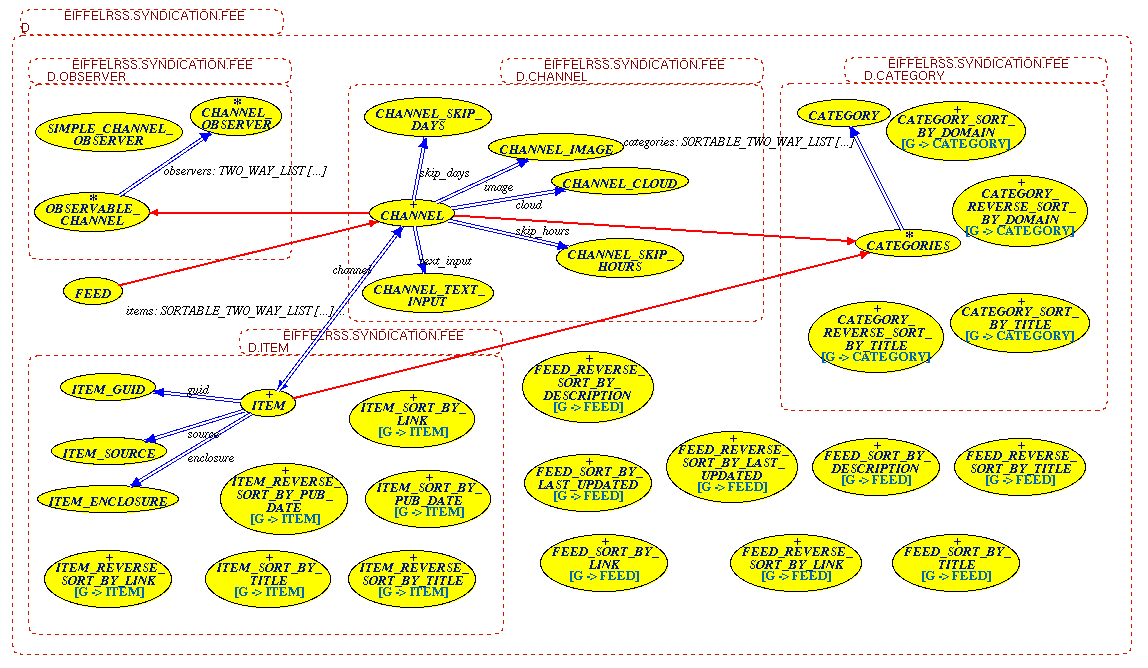
\includegraphics[width=\textwidth]{./figures/EIFFELRSS_SYNDICATION_FEED}
  \caption{BON diagram of cluster \texttt{FEED}}
  \label{fig:feed}
\end{figure}


\chapter{Usage}
\label{cha:feed-usage}

\begin{lstlisting}[language=Eiffel]
class
  FEED_EXAMPLE

create
  make

feature -- Initialization

  make is
      -- Creation procedure.
    do
      -- Create a simple feed with some categories
      create feed.make ("EiffelRSS", create {HTTP_URL}.make ("http://eiffelrss.berlios.de"), "EiffelRSS news")
      feed.add_category (create {CATEGORY}.make_title ("RSS"))
      feed.add_category (create {CATEGORY}.make_title ("Programming"))
      feed.add_category (create {CATEGORY}.make_title ("Eiffel"))
      
      -- Add a cloud to feed
      feed.create_cloud ("eiffelrss.berlios.de", 80, "/RPC2", "xmlStorageSystem.rssPleaseNotify", "xml-rpc")
      
      -- Add an image to feed
      feed.create_image (create {HTTP_URL}.make ("http://eiffelrss.berlios.de/logo.png"), "EiffelRSS", create {HTTP_URL}.make ("http://eiffelrss.berlios.de"))
      
      -- Add a text input field to feed
      feed.create_text_input ("Search", "Search award-winning pages", "search", create {HTTP_URL}.make ("http://eiffelrss.berlios.de/Main/SearchWiki/"))
      
      -- Add some simple items, use `feed.last_added_item' or directly create an item for finer control
      feed.new_item ("Version 23 released!", create {HTTP_URL}.make ("http://eiffelrss.berlios.de/Main/News"), "Version 23 of EiffelRSS got release today. Happy syndicating!")
      feed.last_added_item.add_category (create {CATEGORY}.make_title_domain ("News", create {HTTP_URL}.make ("http://eiffelrss.berlios.de/Main/News/")))
      
      feed.new_item ("EiffelRSS wins award", create {HTTP_URL}.make ("http://eiffelrss.berlios.de/Main/Awards"), "EiffelRSS has been awarded by ISE as best syndication software written in Eiffel. For more info see award-winning pages: http://eiffelrss.berlios.de")
      feed.last_added_item.set_guid (create {ITEM_GUID}.make_perma_link ("http://eiffelrss.berlios.de/newsItem42"))
        
      -- Print feed
      io.put_string ("Sample feed:%N")
      io.put_string ("============%N%N%N")
      io.put_string (feed.to_string)
    end
    
feature -- Arguments

  feed: FEED
      -- Example feed

end -- class FEED_EXAMPLE
\end{lstlisting}


\chapter{Class FEED}
\label{sec:feed-feed}


\section{Overview}
\label{sec:feed-overview}

\texttt{FEED} implements an abstract syndication feed.


\section{Features}
\label{sec:feed-features}

\texttt{FEED} inherits from \texttt{CHANNEL}, so all the
features of \texttt{CHANNEL} are availabe as well.

\subsection{Initialization}
\label{sec:feed-initialization}

\subsubsection{make\_from\_channel}

\begin{lstlisting}[language=Eiffel]
make_from_channel (a_channel: CHANNEL)
  -- Create a new feed from an existing channel
\end{lstlisting}

\subsection{Access}
\label{sec:feed-access}

\subsubsection{last\_updated}

\begin{lstlisting}[language=Eiffel]
last_updated: DATE_TIME
  -- Time the channel was last updated
\end{lstlisting}

\subsubsection{refresh\_period}

\begin{lstlisting}[language=Eiffel]
refresh_period: INTEGER
  -- Refresh period in minutes
\end{lstlisting}


\subsection{Setter}
\label{sec:feed-setter}

\subsubsection{set\_channel}

\begin{lstlisting}[language=Eiffel]
set_channel (a_channel: CHANNEL)
  -- Set channel
\end{lstlisting}

\subsubsection{set\_refresh\_period}

\begin{lstlisting}[language=Eiffel]
set_refresh_period (a_refresh_period: INTEGER)
  -- Set refresh periode in minutes
\end{lstlisting}

\subsubsection{set\_last\_updated}

\begin{lstlisting}[language=Eiffel]
set_last_updated (date: DATE_TIME)
  -- Set time this channel was last updated
\end{lstlisting}


\subsection{Status}
\label{sec:feed-status}

\subsubsection{has\_refresh\_period}

\begin{lstlisting}[language=Eiffel]
has_refresh_period: BOOLEAN
  -- Is `refresh_period' set?
\end{lstlisting}

\subsubsection{has\_last\_updated}

\begin{lstlisting}[language=Eiffel]
has_last_updated: BOOLEAN
  -- Is `last_updated' set?
\end{lstlisting}

\subsubsection{is\_outdated}

\begin{lstlisting}[language=Eiffel]
is_outdated: BOOLEAN
  -- Is the feed outdated?
\end{lstlisting}

\subsubsection{is\_outdated\_default}

\begin{lstlisting}[language=Eiffel]
is_outdated_default (default_refresh_period: INTEGER) : BOOLEAN
  -- Is the feed outdated? 
  -- Use either `refresh_period' or `default_refresh_period' to determine
  -- whether the feed is outdated.
\end{lstlisting}


\subsection{Basic operations}
\label{sec:feed-basic-operations}

\subsubsection{create\_cloud}

\begin{lstlisting}[language=Eiffel]
create_cloud (a_domain: STRING; a_port: INTEGER; a_path: STRING; a_register_procedure: STRING; a_protocol: STRING)
  -- Create and add a cloud
\end{lstlisting}

\subsubsection{create\_image}

\begin{lstlisting}[language=Eiffel]
create_image (a_url: URL; a_title: STRING; a_link: URL)
  -- Create and add an image with URL, title, and link
\end{lstlisting}

\subsubsection{create\_text\_input}

\begin{lstlisting}[language=Eiffel]
create_text_input (a_title: STRING; a_description: STRING; a_name: STRING; a_link: URL)
  -- Create and add a text input with URL, title, and link
\end{lstlisting}

\subsubsection{new\_item}

\begin{lstlisting}[language=Eiffel]
new_item (a_title: STRING; a_link: URL; a_description: STRING)
  -- Create an item with title, link and description
\end{lstlisting}

\subsection{Debug}
\label{sec:feed-debug}

\subsubsection{to\_string}

\begin{lstlisting}[language=Eiffel]
to_string: STRING
  -- Returns a string representation of feed
  -- This feature is especially useful for debugging
\end{lstlisting}


\chapter{Class CHANNEL}
\label{sec:feed-channel}


\section{Overview}
\label{sec:feed-channel-overview}

\texttt{CHANNEL} is a class for abstract syndication channels. It uses
the subclasses \texttt{CHANNEL\_CLOUD}, \texttt{CHANNEL\_IMAGE} and
\texttt{CHANNEL\_TEXT\_INPUT}.


\section{Features}
\label{sec:feed-channel-features}

\subsection{Initialization}
\label{sec:channel-initialization}

\subsubsection{make}

\begin{lstlisting}[language=Eiffel]
make (a_title: STRING; a_link: URL; a_description: STRING)
  --  Create a channel with title, link and description
\end{lstlisting}

\subsection{Access}
\label{sec:channel-access}

\subsubsection{title}

\begin{lstlisting}[language=Eiffel]
title: STRING
  -- Channel title
\end{lstlisting}

\subsubsection{link}

\begin{lstlisting}[language=Eiffel]
link: URL
  -- Channel link
\end{lstlisting}

\subsubsection{description}

\begin{lstlisting}[language=Eiffel]
description: STRING
  -- Channel description
\end{lstlisting}

\subsubsection{language}

\begin{lstlisting}[language=Eiffel]
language: STRING
  -- Channel language
\end{lstlisting}

\subsubsection{copyright}

\begin{lstlisting}[language=Eiffel]
copyright: STRING
  -- Channel copyright
\end{lstlisting}

\subsubsection{managing\_editor}

\begin{lstlisting}[language=Eiffel]
managing_editor: STRING
  -- Channel managing editor
\end{lstlisting}

\subsubsection{web\_master}

\begin{lstlisting}[language=Eiffel]
web_master: STRING
  -- Channel web master
\end{lstlisting}

\subsubsection{pub\_date}

\begin{lstlisting}[language=Eiffel]
pub_date: DATE_TIME
  -- Channel pulication date
\end{lstlisting}

\subsubsection{last\_build\_date}

\begin{lstlisting}[language=Eiffel]
last_build_date: DATE_TIME
  -- Channel last build date
\end{lstlisting}

\subsubsection{feed\_generator}

\begin{lstlisting}[language=Eiffel]
feed_generator: STRING
  -- Channel feed generator
\end{lstlisting}

\subsubsection{docs}

\begin{lstlisting}[language=Eiffel]
docs: URL
  -- Channel docs
\end{lstlisting}

\subsubsection{cloud}

\begin{lstlisting}[language=Eiffel]
cloud: CHANNEL_CLOUD
  -- Channel cloud
\end{lstlisting}

\subsubsection{ttl}

\begin{lstlisting}[language=Eiffel]
ttl: INTEGER
  -- Channel time to live in minutes
\end{lstlisting}

\subsubsection{image}

\begin{lstlisting}[language=Eiffel]
image: CHANNEL_IMAGE
  -- Channel image
\end{lstlisting}

\subsubsection{text\_input}

\begin{lstlisting}[language=Eiffel]
text_input: CHANNEL_TEXT_INPUT
  -- Channel text input
\end{lstlisting}

\subsubsection{skip\_hours}

\begin{lstlisting}[language=Eiffel]
skip_hours: CHANNEL_SKIP_HOURS
  -- Channel skip hours
\end{lstlisting}

\subsubsection{skip\_days}

\begin{lstlisting}[language=Eiffel]
skip_days: CHANNEL_SKIP_DAYS
  -- Channel skip days
\end{lstlisting}

\subsubsection{items}

\begin{lstlisting}[language=Eiffel]
items: SORTABLE_TWO_WAY_LIST[ITEM]
  -- Channel items
\end{lstlisting}

\subsection{Access (RSS 0.91)}
\label{sec:channel-access-rss091}

\subsubsection{rating}

\begin{lstlisting}[language=Eiffel]
rating: STRING
  -- Channel rating
\end{lstlisting}

\subsection{Access (RSS 1.0)}
\label{sec:channel-access-rss10}

\subsubsection{items\_toc}

\begin{lstlisting}[language=Eiffel]
items_toc: TWO_WAY_LIST[URL]
  -- Channel items table of content
\end{lstlisting}

\subsubsection{textinput}

\begin{lstlisting}[language=Eiffel]
textinput: URL
  -- Channel textinput URL
\end{lstlisting}


\subsection{Access (categories)}
\label{sec:channel-access-categories}

\subsubsection{categories}

\begin{lstlisting}[language=Eiffel]
categories: SORTABLE_TWO_WAY_LIST[CATEGORY]
  -- Categories list containing category items
\end{lstlisting}

\subsection{Access (observers)}
\label{sec:channel-access-observer}

\subsubsection{observers}

\begin{lstlisting}[language=Eiffel]
observers: TWO_WAY_LIST[CHANNEL_OBSERVER]
  -- List of subscribed observers
\end{lstlisting}


\subsection{Access (metadata)}
\label{sec:channel-access-metadata}

\subsubsection{last\_added\_item}

\begin{lstlisting}[language=Eiffel]
last_added_item: ITEM
  -- The last added channel item
\end{lstlisting}

\subsection{Setter}
\label{sec:channel-setter}

\subsubsection{set\_title}

\begin{lstlisting}[language=Eiffel]
set_title (a_title: STRING)
  -- Set title to `a_title'
\end{lstlisting}

\subsubsection{set\_link}

\begin{lstlisting}[language=Eiffel]
set_link (a_link: URL)
  -- Set link to `a_link'
\end{lstlisting}

\subsubsection{set\_description}

\begin{lstlisting}[language=Eiffel]
set_description (a_description: STRING)
  -- Set description to `a_description'
\end{lstlisting}

\subsubsection{set\_language}

\begin{lstlisting}[language=Eiffel]
set_language (a_language: STRING)
  -- Channel language
\end{lstlisting}

\subsubsection{set\_copyright}

\begin{lstlisting}[language=Eiffel]
set_copyright (a_copyright: STRING)
  -- Channel copyright
\end{lstlisting}

\subsubsection{set\_managing\_editor}

\begin{lstlisting}[language=Eiffel]
set_managing_editor (a_managing_editor: STRING)
  -- Channel managing editor
\end{lstlisting}

\subsubsection{set\_web\_master}

\begin{lstlisting}[language=Eiffel]
set_web_master (a_web_master: STRING)
  -- Channel web master
\end{lstlisting}

\subsubsection{set\_pub\_date}

\begin{lstlisting}[language=Eiffel]
set_pub_date (date: DATE_TIME)
  -- Channel pulication date
\end{lstlisting}

\subsubsection{set\_last\_build\_date}

\begin{lstlisting}[language=Eiffel]
set_last_build_date (date: DATE_TIME)
  -- Channel last build date
\end{lstlisting}

\subsubsection{set\_feed\_generator}

\begin{lstlisting}[language=Eiffel]
set_feed_generator (a_feed_generator: STRING)
  -- Channel feed generator
\end{lstlisting}

\subsubsection{set\_docs}

\begin{lstlisting}[language=Eiffel]
set_docs (url: URL)
  -- Channel docs
\end{lstlisting}

\subsubsection{set\_cloud}

\begin{lstlisting}[language=Eiffel]
set_cloud (a_cloud: CHANNEL_CLOUD)
  -- Channel cloud
\end{lstlisting}

\subsubsection{set\_ttl}

\begin{lstlisting}[language=Eiffel]
set_ttl (a_ttl: INTEGER)
  -- Channel time to live in minutes
\end{lstlisting}

\subsubsection{set\_image}

\begin{lstlisting}[language=Eiffel]
set_image (an_image: CHANNEL_IMAGE)
  -- Channel image
\end{lstlisting}

\subsubsection{set\_text\_input}

\begin{lstlisting}[language=Eiffel]
set_text_input (a_text_input: CHANNEL_TEXT_INPUT)
  -- Channel text input
\end{lstlisting}

\subsubsection{set\_skip\_hours}

\begin{lstlisting}[language=Eiffel]
set_skip_hours (some_skip_hours: CHANNEL_SKIP_HOURS)
  -- Channel skip hours
\end{lstlisting}

\subsubsection{set\_skip\_days}

\begin{lstlisting}[language=Eiffel]
set_skip_days (some_skip_days: CHANNEL_SKIP_DAYS)
  -- Channel skip days 
\end{lstlisting}

\subsubsection{set\_items}

\begin{lstlisting}[language=Eiffel]
set_items (item_list: like items)
  -- Channel items
\end{lstlisting}

\subsection{Setter (RSS 0.91)}
\label{sec:channel-setter-rss091}

\subsubsection{set\_rating}

\begin{lstlisting}[language=Eiffel]
set_rating (rating_value: STRING)
  -- Channel rating
\end{lstlisting}

\subsection{Setter (RSS 1.0)}
\label{sec:channel-setter-rss10}

\subsubsection{set\_items\_toc}

\begin{lstlisting}[language=Eiffel]
set_items_toc (item_toc_list: like items_toc)
  -- Channel items table of content 
\end{lstlisting}

\subsubsection{set\_textinput}

\begin{lstlisting}[language=Eiffel]
set_textinput (url: URL)
  -- Channel textinput URL
\end{lstlisting}

\subsection{Setter (categories)}
\label{sec:channel-setter-categories}

\subsubsection{set\_categories}

\begin{lstlisting}[language=Eiffel]
set_categories (category_list: like categories)
  -- Set categories with a new category list
\end{lstlisting}

\subsection{Setter (observers)}
\label{sec:channel-setter-observer}

\subsubsection{set\_observers}

\begin{lstlisting}[language=Eiffel]
set_observers (observer_list: like observers)
  -- List of subscribed observers
\end{lstlisting}


\subsection{Status}
\label{sec:channel-status}

\subsubsection{has\_language}

\begin{lstlisting}[language=Eiffel]
has_language: BOOLEAN
  -- Is `language' set and non-empty?
\end{lstlisting}

\subsubsection{has\_copyright}

\begin{lstlisting}[language=Eiffel]
has_copyright: BOOLEAN
  -- Is `copyright' set and non-empty?
\end{lstlisting}

\subsubsection{has\_managing\_editor}

\begin{lstlisting}[language=Eiffel]
has_managing_editor: BOOLEAN
  -- Is `managing_editor' set and non-empty?
\end{lstlisting}

\subsubsection{has\_web\_master}

\begin{lstlisting}[language=Eiffel]
has_web_master: BOOLEAN
  -- Is `web_master' set and non-empty?
\end{lstlisting}

\subsubsection{has\_pub\_date}

\begin{lstlisting}[language=Eiffel]
has_pub_date: BOOLEAN
  -- Is `pub_date' set?
\end{lstlisting}

\subsubsection{has\_last\_build\_date}

\begin{lstlisting}[language=Eiffel]
has_last_build_date: BOOLEAN
  -- Is `last_build_date' set?
\end{lstlisting}

\subsubsection{has\_feed\_generator}

\begin{lstlisting}[language=Eiffel]
has_feed_generator: BOOLEAN
  -- Is `feed_generator' set and non-empty?
\end{lstlisting}

\subsubsection{has\_docs}

\begin{lstlisting}[language=Eiffel]
has_docs: BOOLEAN
  -- Is `docs' set?
\end{lstlisting}

\subsubsection{has\_cloud}

\begin{lstlisting}[language=Eiffel]
has_cloud: BOOLEAN
  -- Is `cloud' set?
\end{lstlisting}

\subsubsection{has\_ttl}

\begin{lstlisting}[language=Eiffel]
has_ttl: BOOLEAN
  -- Is `ttl' set?
\end{lstlisting}

\subsubsection{has\_image}

\begin{lstlisting}[language=Eiffel]
has_image: BOOLEAN
  -- Is `image' set?
\end{lstlisting}

\subsubsection{has\_text\_input}

\begin{lstlisting}[language=Eiffel]
has_text_input: BOOLEAN
  -- Is `text_input' set?
\end{lstlisting}

\subsubsection{has\_skip\_hours}

\begin{lstlisting}[language=Eiffel]
has_skip_hours: BOOLEAN
  -- Is `skip_hours' set?
\end{lstlisting}

\subsubsection{has\_skip\_days}

\begin{lstlisting}[language=Eiffel]
has_skip_days: BOOLEAN
  -- Is `skip_days' set?
\end{lstlisting}

\subsubsection{has\_items}

\begin{lstlisting}[language=Eiffel]
has_items: BOOLEAN
  -- Is `items' set?
\end{lstlisting}

\subsection{Status (RSS 0.91)}
\label{sec:channel-status-rss091}

\subsubsection{has\_rating}

\begin{lstlisting}[language=Eiffel]
has_rating: BOOLEAN
  -- Is `rating' set and non-empty?
\end{lstlisting}

\subsection{Status (RSS 1.0)}
\label{sec:channel-status-rss10}

\subsubsection{has\_items\_toc}

\begin{lstlisting}[language=Eiffel]
has_items_toc: BOOLEAN
  -- Is `items_toc' set?
\end{lstlisting}

\subsubsection{has\_textinput}

\begin{lstlisting}[language=Eiffel]
has_textinput: BOOLEAN
  -- Is `textinput' set?
\end{lstlisting}

\subsection{Status (categories)}
\label{sec:channel-status-categories}

\subsubsection{has\_categories}

\begin{lstlisting}[language=Eiffel]
has_categories: BOOLEAN
  -- Are there any categories?
\end{lstlisting}

\subsection{Status (observers)}
\label{sec:channel-status-observer}

\subsubsection{has\_observers}

\begin{lstlisting}[language=Eiffel]
has_observers: BOOLEAN
  -- Is `observers' set?
\end{lstlisting}


\subsection{Status (metadata)}
\label{sec:channel-status-metadata}

\subsubsection{has\_last\_added\_item}

\begin{lstlisting}[language=Eiffel]
has_last_added_item: BOOLEAN
  -- Is `last_added_item' set?
\end{lstlisting}

\subsection{Basic operations}
\label{sec:channel-basic-operations}

\subsubsection{add\_skip\_hour}

\begin{lstlisting}[language=Eiffel]
add_skip_hour (skip_hour: INTEGER)
  -- Add a skip hour.
  -- Only 0 <= `skip_hour' <= 23 is valid
\end{lstlisting}

\subsubsection{remove\_skip\_hour}

\begin{lstlisting}[language=Eiffel]
remove_skip_hour (skip_hour: INTEGER)
  -- Remove a skip hour
\end{lstlisting}

\subsubsection{add\_skip\_day}

\begin{lstlisting}[language=Eiffel]
add_skip_day (skip_day: STRING)
  -- Add a skip day.
  -- `skip_day' will be added to `skip_days' with the first letter to upper
  -- and the rest to lower. For example: `mOnDaY' is added as `Monday'
\end{lstlisting}

\subsubsection{remove\_skip\_day}

\begin{lstlisting}[language=Eiffel]
remove_skip_day (skip_day: STRING)
  -- Remove a skip day
\end{lstlisting}

\subsubsection{add\_item}

\begin{lstlisting}[language=Eiffel]
add_item (item: ITEM)
  -- Add an item
\end{lstlisting}

\subsubsection{remove\_item}

\begin{lstlisting}[language=Eiffel]
remove_item (item: ITEM)
  -- Remove an item
\end{lstlisting}

\subsection{Basic operations (RSS 0.91)}
\label{sec:channel-basic-operations-rss091}

\subsubsection{}

\begin{lstlisting}[language=Eiffel]
\end{lstlisting}

\subsection{Basic operations (RSS 1.0)}
\label{sec:channel-basic-operations-rss10}

\subsubsection{add\_item\_toc}

\begin{lstlisting}[language=Eiffel]
add_item_toc (item_toc: URL)
  -- Add an item to the TOC  
\end{lstlisting}

\subsubsection{remove\_item\_toc}

\begin{lstlisting}[language=Eiffel]
remove_item_toc (item_toc: URL)
  -- Remove an item from the TOC
\end{lstlisting}

\subsection{Basic operations (categories)}
\label{sec:channel-basic-operations-categories}

\subsubsection{add\_category}

\begin{lstlisting}[language=Eiffel]
add_category (category: CATEGORY)
  -- Add a category item
\end{lstlisting}

\subsubsection{remove\_category}

\begin{lstlisting}[language=Eiffel]
remove_category (category: CATEGORY)
  -- Remove a category item
\end{lstlisting}

\subsection{Basic operations (observers)}
\label{sec:channel-basic-operations-observer}

\subsubsection{add\_observer}

\begin{lstlisting}[language=Eiffel]
add_observer (an_observer: CHANNEL_OBSERVER)
  -- Add an observer
\end{lstlisting}

\subsubsection{remove\_observer}

\begin{lstlisting}[language=Eiffel]
remove_observer (an_observer: CHANNEL_OBSERVER)
  -- Remove an observer
\end{lstlisting}

\subsection{Sort}
\label{sec:channel-sort}

\subsubsection{sort\_items\_by\_title}

\begin{lstlisting}[language=Eiffel]
sort_items_by_title
  -- Sort items by title
\end{lstlisting}

\subsubsection{sort\_items\_by\_pub\_date}

\begin{lstlisting}[language=Eiffel]
sort_items_by_pub_date
  -- Sort items by publication date
\end{lstlisting}

\subsubsection{sort\_items\_by\_link}

\begin{lstlisting}[language=Eiffel]
sort_items_by_link
  -- Sort items by link
\end{lstlisting}

\subsubsection{reverse\_sort\_items\_by\_title}

\begin{lstlisting}[language=Eiffel]
reverse_sort_items_by_title
  -- Reverse sort items by title
\end{lstlisting}

\subsubsection{reverse\_sort\_items\_by\_pub\_date}

\begin{lstlisting}[language=Eiffel]
reverse_sort_items_by_pub_date
  -- Reverse sort items by publication date
\end{lstlisting}

\subsubsection{reverse\_sort\_items\_by\_link}

\begin{lstlisting}[language=Eiffel]
reverse_sort_items_by_link
  -- Reverse sort items by link
\end{lstlisting}

\subsection{Sort (categories)}
\label{sec:channel-sort-categories}

\subsubsection{sort\_categories\_by\_title}

\begin{lstlisting}[language=Eiffel]
sort_categories_by_title
  -- Sort categories by title
\end{lstlisting}

\subsubsection{sort\_categories\_by\_domain}

\begin{lstlisting}[language=Eiffel]
sort_categories_by_domain
  -- Sort categories by domain
\end{lstlisting}

\subsubsection{reverse\_sort\_categories\_by\_title}

\begin{lstlisting}[language=Eiffel]
reverse_sort_categories_by_title
  -- Reverse sort categories by title
\end{lstlisting}

\subsubsection{reverse\_sort\_categories\_by\_domain}

\begin{lstlisting}[language=Eiffel]
reverse_sort_categories_by_domain
  -- Reverse sort categories by domain
\end{lstlisting}


\subsection{Debug}
\label{sec:channel-debug}

\subsubsection{to\_string}

\begin{lstlisting}[language=Eiffel]
to_string: STRING
  -- Returns a string representation of channel
  -- This feature is especially useful for debugging
\end{lstlisting}


\section{Subclass CHANNEL\_CLOUD}
\label{sec:channel-cloud}

\subsection{Initialization}
\label{sec:channel-cloud-initialization}

\subsubsection{make}

\begin{lstlisting}[language=Eiffel]
make (a_domain: STRING; a_port: INTEGER; a_path: STRING; a_register_procedure: STRING; a_protocol: STRING)
  -- Create a channel cloud with domain, port, path, register procedure and protocol
\end{lstlisting}

\subsection{Access}
\label{sec:channel-cloud-access}

\subsubsection{domain}

\begin{lstlisting}[language=Eiffel]
domain: STRING
  -- Domain of the cloud
\end{lstlisting}

\subsubsection{port}

\begin{lstlisting}[language=Eiffel]
port: INTEGER
  -- Port of the cloud
\end{lstlisting}

\subsubsection{path}

\begin{lstlisting}[language=Eiffel]
path: STRING
  -- Path of the cloud
\end{lstlisting}

\subsubsection{register\_procedure}

\begin{lstlisting}[language=Eiffel]
register_procedure: STRING
  -- Register procedure of the cloud
\end{lstlisting}

\subsubsection{protocol}

\begin{lstlisting}[language=Eiffel]
protocol: STRING
  -- Protocol of the cloud
\end{lstlisting}

\subsection{Setter}
\label{sec:channel-cloud-setter}

\subsubsection{set\_domain}

\begin{lstlisting}[language=Eiffel]
set_domain (a_domain: STRING)
  -- Set domain to`a_domain'
\end{lstlisting}

\subsubsection{set\_port}

\begin{lstlisting}[language=Eiffel]
set_port (a_port: INTEGER)
  -- Set port to `a_port'
\end{lstlisting}

\subsubsection{set\_path}

\begin{lstlisting}[language=Eiffel]
set_path (a_path: STRING)
  -- Set path to `a_path'
\end{lstlisting}

\subsubsection{set\_register\_procedure}

\begin{lstlisting}[language=Eiffel]
set_register_procedure (a_register_procedure: STRING)
  -- Set register_procedure to `a_register_procedure'
\end{lstlisting}

\subsubsection{set\_protocol}

\begin{lstlisting}[language=Eiffel]
set_protocol (a_protocol: STRING)
  -- Set protocol to `a_protocol'
\end{lstlisting}

\subsection{Debug}
\label{sec:channel-cloud-debug}

\subsubsection{to\_string}

\begin{lstlisting}[language=Eiffel]
to_string: STRING is
  -- Returns a string representation of cloud
  -- This feature is especially useful for debugging
\end{lstlisting}


\section{Subclass CHANNEL\_IMAGE}
\label{sec:channel-image}

\subsection{Initialization}
\label{sec:channel-image-initialization}

\subsubsection{make}

\begin{lstlisting}[language=Eiffel]
make (a_url: URL; a_title: STRING; a_link: URL)
  -- Create a channel image with URL, title, and link
\end{lstlisting}

\subsection{Constants}
\label{sec:channel-image-constants}

\subsubsection{Default\_width}

\begin{lstlisting}[language=Eiffel]
Default_width: INTEGER is 88
  -- Default width of the image
\end{lstlisting}

\subsubsection{Max\_width}

\begin{lstlisting}[language=Eiffel]
Max_width: INTEGER is 144
  -- Maximum width of the image
\end{lstlisting}

\subsection{Access}
\label{sec:channel-image-access}

\subsubsection{url}

\begin{lstlisting}[language=Eiffel]
url: URL
  -- URL of the image
\end{lstlisting}

\subsubsection{title}

\begin{lstlisting}[language=Eiffel]
title: STRING
  -- Title of the image
\end{lstlisting}

\subsubsection{link}

\begin{lstlisting}[language=Eiffel]
link: URL
  -- Link of the image
\end{lstlisting}

\subsubsection{width, height}

\begin{lstlisting}[language=Eiffel]
width, height: INTEGER
  -- Width and height of the image
\end{lstlisting}

\subsubsection{description}

\begin{lstlisting}[language=Eiffel]
description: STRING
  -- Description of the image
\end{lstlisting}

\subsection{Setter}
\label{sec:channel-image-setter}

\subsubsection{set\_url}

\begin{lstlisting}[language=Eiffel]
set_url (a_url: URL)
  -- Set url to`a_url'
\end{lstlisting}

\subsubsection{set\_title}

\begin{lstlisting}[language=Eiffel]
set_title (a_title: STRING)
  -- Set title to`a_title'
\end{lstlisting}

\subsubsection{set\_link}

\begin{lstlisting}[language=Eiffel]
set_link (a_link: URL)
  -- Set link to`a_link'
\end{lstlisting}

\subsubsection{set\_width}

\begin{lstlisting}[language=Eiffel]
set_width (a_width: INTEGER)
  -- Set width to`a_width'
\end{lstlisting}

\subsubsection{set\_height}

\begin{lstlisting}[language=Eiffel]
set_height (a_height: INTEGER)
  -- Set heigh to`a_heigh'
\end{lstlisting}

\subsubsection{set\_description}

\begin{lstlisting}[language=Eiffel]
set_description (a_description: STRING)
  -- Set  to`a_description'
\end{lstlisting}

\subsection{Status}
\label{sec:channel-image-status}

\subsubsection{has\_width}

\begin{lstlisting}[language=Eiffel]
has_width: BOOLEAN
  -- Is `width' set?
\end{lstlisting}

\subsubsection{has\_height}

\begin{lstlisting}[language=Eiffel]
has_height: BOOLEAN
  -- Is `height' set?
\end{lstlisting}

\subsubsection{has\_description}

\begin{lstlisting}[language=Eiffel]
has_description: BOOLEAN
  -- Is `description' set and non-empty?
\end{lstlisting}

\subsection{Debug}
\label{sec:channel-image-debug}

\subsubsection{to\_string}

\begin{lstlisting}[language=Eiffel]
to_string: STRING
  -- Returns a string representation of image
  -- This feature is especially useful for debugging
\end{lstlisting}

\section{Subclass CHANNEL\_TEXT\_INPUT}
\label{sec:channel-text-input}

\subsection{Initialization}
\label{sec:channel-text-input-initialization}

\subsubsection{make}

\begin{lstlisting}[language=Eiffel]
make (a_title: STRING; a_description: STRING; a_name: STRING; a_link: URL)
  -- Create a channel text input with title, description, name and link
\end{lstlisting}

\subsection{Access}
\label{sec:channel-text-input-access}

\subsubsection{title}

\begin{lstlisting}[language=Eiffel]
title: STRING
  -- Title of the text input
\end{lstlisting}

\subsubsection{description}

\begin{lstlisting}[language=Eiffel]
description: STRING
  -- Description of the text input
\end{lstlisting}

\subsubsection{name}

\begin{lstlisting}[language=Eiffel]
name: STRING
  -- Name of the text input
\end{lstlisting}

\subsubsection{link}

\begin{lstlisting}[language=Eiffel]
link: URL
  -- Link of the text input
\end{lstlisting}

\subsection{Setter}
\label{sec:channel-text-input-setter}

\subsubsection{set\_title}

\begin{lstlisting}[language=Eiffel]
set_title (a_title: STRING)
  -- Set title to`a_title'
\end{lstlisting}

\subsubsection{set\_description}

\begin{lstlisting}[language=Eiffel]
set_description (a_description: STRING)
  -- Set description to`a_description'
\end{lstlisting}

\subsubsection{set\_name}

\begin{lstlisting}[language=Eiffel]
set_name (a_name: STRING)
  -- Set name to`a_name'
\end{lstlisting}

\subsubsection{set\_link}

\begin{lstlisting}[language=Eiffel]
set_link (a_link: URL)
  -- Set link to`a_link'
\end{lstlisting}

\subsection{Debug}
\label{sec:channel-text-input-debug}

\subsubsection{to\_string}

\begin{lstlisting}[language=Eiffel]
to_string: STRING is
  -- Returns a string representation of text input
  -- This feature is especially useful for debugging
\end{lstlisting}


\chapter{Class ITEM}
\label{sec:feed-item}


\section{Overview}
\label{sec:feed-item-overview}

\texttt{ITEM} is a class for feed items. It uses the subclasses
\texttt{ITEM\_ENCLOSURE}, \texttt{ITEM\_GUID} and \texttt{ITEM\_SOURCE}.


\section{Features}
\label{sec:feed-item-features}


\subsection{Initialization}
\label{sec:item-initialization}

\subsubsection{make}

\begin{lstlisting}[language=Eiffel]
make (a_channel: CHANNEL; a_title: STRING; a_link: URL; a_description: STRING)
  -- Create an item with title, link and description
\end{lstlisting}

\subsubsection{make\_title}

\begin{lstlisting}[language=Eiffel]
make_title (a_channel: CHANNEL; a_title: STRING)
  -- Create an item with title
\end{lstlisting}

\subsubsection{make\_description}

\begin{lstlisting}[language=Eiffel]
make_description (a_channel: CHANNEL; a_description: STRING)
  -- Create an item with description
\end{lstlisting}

\subsection{Access}
\label{sec:item-access}

\subsubsection{channel}

\begin{lstlisting}[language=Eiffel]
channel: CHANNEL
  -- Backlink to the corresponding channel
\end{lstlisting}

\subsubsection{title}

\begin{lstlisting}[language=Eiffel]
title: STRING
  -- Item title
\end{lstlisting}

\subsubsection{link}

\begin{lstlisting}[language=Eiffel]
link: URL
  -- Item link
\end{lstlisting}

\subsubsection{description}

\begin{lstlisting}[language=Eiffel]
description: STRING
  -- Item description
\end{lstlisting}

\subsubsection{author}

\begin{lstlisting}[language=Eiffel]
author: STRING
  -- Item author
\end{lstlisting}

\subsubsection{comments}

\begin{lstlisting}[language=Eiffel]
comments: URL
  -- Item comment URL
\end{lstlisting}

\subsubsection{enclosure}

\begin{lstlisting}[language=Eiffel]
enclosure: ITEM_ENCLOSURE
  -- Item enclosure
\end{lstlisting}

\subsubsection{guid}

\begin{lstlisting}[language=Eiffel]
guid: ITEM_GUID
  -- Item globally unique identifier (guid)
\end{lstlisting}

\subsubsection{pub\_date}

\begin{lstlisting}[language=Eiffel]
pub_date: DATE_TIME
  -- Item publication date
\end{lstlisting}

\subsubsection{source}

\begin{lstlisting}[language=Eiffel]
source: ITEM_SOURCE
  -- Item source
\end{lstlisting}


\subsection{Access (categories)}
\label{sec:item-access-categories}

\subsubsection{categories}

\begin{lstlisting}[language=Eiffel]
categories: SORTABLE_TWO_WAY_LIST[CATEGORY]
  -- Categories list containing category items
\end{lstlisting}

\subsection{Access (metadata)}
\label{sec:item-access-metadata}

\subsubsection{date\_found}

\begin{lstlisting}[language=Eiffel]
date_found: DATE_TIME
  -- Item date found
\end{lstlisting}

\subsubsection{is\_read}

\begin{lstlisting}[language=Eiffel]
is_read: BOOLEAN
  -- Is the item read?
\end{lstlisting}

\subsection{Setter}
\label{sec:item-setter}

\subsubsection{set\_channel}

\begin{lstlisting}[language=Eiffel]
set_channel (a_channel: CHANNEL)
  -- Set channel to `a_channel'
\end{lstlisting}

\subsubsection{set\_title}

\begin{lstlisting}[language=Eiffel]
set_title (a_title: STRING)
  -- Set title to `a_title'
\end{lstlisting}

\subsubsection{set\_link}

\begin{lstlisting}[language=Eiffel]
set_link (a_link: URL)
  -- Set link to `a_link'
\end{lstlisting}

\subsubsection{set\_description}

\begin{lstlisting}[language=Eiffel]
set_description (a_description: STRING)
  -- Set description to `a_description'
\end{lstlisting}

\subsubsection{set\_author}

\begin{lstlisting}[language=Eiffel]
set_author (an_author: STRING)
  -- Set author to `an_author'
\end{lstlisting}

\subsubsection{set\_comments}

\begin{lstlisting}[language=Eiffel]
set_comments (url: URL)
  -- Set comments to `url'
\end{lstlisting}

\subsubsection{set\_enclosure}

\begin{lstlisting}[language=Eiffel]
set_enclosure (an_enclosure: ITEM_ENCLOSURE)
  -- Set enclosure to `an_enclosure'
\end{lstlisting}

\subsubsection{set\_guid}

\begin{lstlisting}[language=Eiffel]
set_guid (a_guid: ITEM_GUID)
  -- Set guid to `a_guid'
\end{lstlisting}

\subsubsection{set\_pub\_date}

\begin{lstlisting}[language=Eiffel]
set_pub_date (date: DATE_TIME)
  -- Set publication date to `date'
\end{lstlisting}

\subsubsection{set\_source}

\begin{lstlisting}[language=Eiffel]
set_source (a_source: ITEM_SOURCE)
  -- Set source to `a_source'
\end{lstlisting}

\subsection{Setter (categories)}
\label{sec:item-setter-categories}

\subsubsection{set\_categories}

\begin{lstlisting}[language=Eiffel]
set_categories (category_list: like categories)
  -- Set categories with a new category list
\end{lstlisting}

\subsection{Setter (metadata)}
\label{sec:item-setter-metadata}

\subsubsection{set\_date\_found}

\begin{lstlisting}[language=Eiffel]
set_date_found (date: DATE_TIME)
  -- Set date_found to `date'
\end{lstlisting}

\subsubsection{set\_read}

\begin{lstlisting}[language=Eiffel]
set_read (value: BOOLEAN)
  -- Set is_read to `value'
\end{lstlisting}

\subsection{Status}
\label{sec:item-status}

\subsubsection{has\_title}

\begin{lstlisting}[language=Eiffel]
has_title: BOOLEAN
  -- Is `title' set and non-empty?
\end{lstlisting}

\subsubsection{has\_link}

\begin{lstlisting}[language=Eiffel]
has_link: BOOLEAN
  -- Is `link' set?
\end{lstlisting}

\subsubsection{has\_description}

\begin{lstlisting}[language=Eiffel]
has_description: BOOLEAN
  -- Is `description' set and non-empty?
\end{lstlisting}

\subsubsection{has\_author}

\begin{lstlisting}[language=Eiffel]
has_author: BOOLEAN
  -- Is `author' set and non-empty?
\end{lstlisting}

\subsubsection{has\_comments}

\begin{lstlisting}[language=Eiffel]
has_comments: BOOLEAN
  -- Is `comments' set?
\end{lstlisting}

\subsubsection{has\_enclosure}

\begin{lstlisting}[language=Eiffel]
has_enclosure: BOOLEAN
  -- Is `enclosure' set?
\end{lstlisting}

\subsubsection{has\_guid}

\begin{lstlisting}[language=Eiffel]
has_guid: BOOLEAN
  -- Is `guid' set?
\end{lstlisting}

\subsubsection{has\_pub\_date}

\begin{lstlisting}[language=Eiffel]
has_pub_date: BOOLEAN
  -- Is `pub_date' set?
\end{lstlisting}

\subsubsection{has\_source}

\begin{lstlisting}[language=Eiffel]
has_source: BOOLEAN
  -- Is `source' set?
\end{lstlisting}

\subsection{Status (categories)}
\label{sec:item-status-categories}

\subsubsection{has\_categories}

\begin{lstlisting}[language=Eiffel]
has_categories: BOOLEAN
  -- Are there any categories?
\end{lstlisting}

\subsection{Basic operations (categories)}
\label{sec:item-basic-operations-categories}

\subsubsection{add\_category}

\begin{lstlisting}[language=Eiffel]
add_category (category: CATEGORY)
  -- Add a category item
\end{lstlisting}

\subsubsection{remove\_category}

\begin{lstlisting}[language=Eiffel]
remove_category (category: CATEGORY)
  -- Remove a category item
\end{lstlisting}

\subsection{Sort (categories)}
\label{sec:item-sort-categories}

\subsubsection{sort\_categories\_by\_title}

\begin{lstlisting}[language=Eiffel]
sort_categories_by_title
  -- Sort categories by title
\end{lstlisting}

\subsubsection{sort\_categories\_by\_domain}

\begin{lstlisting}[language=Eiffel]
sort_categories_by_domain
  -- Sort categories by domain
\end{lstlisting}

\subsubsection{reverse\_sort\_categories\_by\_title}

\begin{lstlisting}[language=Eiffel]
reverse_sort_categories_by_title
  -- Reverse sort categories by title
\end{lstlisting}

\subsubsection{reverse\_sort\_categories\_by\_domain}

\begin{lstlisting}[language=Eiffel]
reverse_sort_categories_by_domain
  -- Reverse sort categories by domain
\end{lstlisting}

\subsection{Debug}
\label{sec:item-debug}

\subsubsection{to\_string}

\begin{lstlisting}[language=Eiffel]
to_string: STRING
  -- Returns a string representation of item
  -- This feature is especially useful for debugging
\end{lstlisting}


\section{Subclass ITEM\_ENCLOSURE}
\label{sec:item-enclosure}

\subsection{Initialization}
\label{sec:item-enclosure-initialization}

\subsubsection{make}

\begin{lstlisting}[language=Eiffel]
make (a_url: URL; a_length: INTEGER; a_type: STRING)
  -- Create an item enclosure
\end{lstlisting}

\subsection{Access}
\label{sec:item-enclosure-access}

\subsubsection{url}

\begin{lstlisting}[language=Eiffel]
url: URL
  -- URL of the enclosure
\end{lstlisting}

\subsubsection{length}

\begin{lstlisting}[language=Eiffel]
length: INTEGER
  -- Length in bytes of the enclosure
\end{lstlisting}

\subsubsection{type}

\begin{lstlisting}[language=Eiffel]
type: STRING
  -- MIME type of the enclosure
\end{lstlisting}

\subsection{Setter}
\label{sec:item-enclosure-setter}

\subsubsection{set\_url}

\begin{lstlisting}[language=Eiffel]
set_url (a_url: URL)
  -- Set the URL to `url'
\end{lstlisting}

\subsubsection{set\_length}

\begin{lstlisting}[language=Eiffel]
set_length (a_length: INTEGER)
  -- Set the length to `a_length'
\end{lstlisting}

\subsubsection{set\_type}

\begin{lstlisting}[language=Eiffel]
set_type (a_type: STRING)
  -- Set the MIME type to `a_type'
\end{lstlisting}

\subsection{Debug}
\label{sec:item-enclosure-debug}

\subsubsection{to\_string}

\begin{lstlisting}[language=Eiffel]
to_string: STRING
  -- Returns a string representation of enclosure
  -- This feature is especially useful for debugging
\end{lstlisting}


\section{Subclass ITEM\_GUID}
\label{sec:item-guid}

\subsection{Initialization}
\label{sec:item-guid-initialization}

\subsubsection{make}

\begin{lstlisting}[language=Eiffel]
make (a_guid: STRING)
  -- Create an item guid with `is_perma_link' set to False
\end{lstlisting}

\subsubsection{make\_perma\_link}

\begin{lstlisting}[language=Eiffel]
make_perma_link (a_guid: STRING)
  -- Create an item guid with `is_perma_link' set to True
\end{lstlisting}

\subsection{Access}
\label{sec:item-guid-access}

\subsubsection{guid}

\begin{lstlisting}[language=Eiffel]
guid: STRING
  -- String representing a globally unique identifier (guid)
\end{lstlisting}

\subsubsection{is\_perma\_link}

\begin{lstlisting}[language=Eiffel]
is_perma_link: BOOLEAN
  -- Is this guid a perma link?
\end{lstlisting}

\subsection{Setter}
\label{sec:item-guid-setter}

\subsubsection{set\_guid}

\begin{lstlisting}[language=Eiffel]
set_guid (a_guid: STRING)
  -- Set guid to `a_guid'
\end{lstlisting}

\subsubsection{set\_perma\_link}

\begin{lstlisting}[language=Eiffel]
set_perma_link (value: BOOLEAN)
  -- Set is_perma_link to `value'
\end{lstlisting}

\subsection{Debug}
\label{sec:item-guid-debug}

\subsubsection{to\_string}

\begin{lstlisting}[language=Eiffel]
to_string: STRING
  -- Returns a string representation of guid
  -- This feature is especially useful for debugging
\end{lstlisting}

\section{Subclass ITEM\_SOURCE}
\label{sec:item-source}

\subsection{Initialization}
\label{sec:item-source-initialization}

\subsubsection{make}

\begin{lstlisting}[language=Eiffel]
make (a_name: STRING; a_url: URL)
  -- Create an item source
\end{lstlisting}

\subsection{Access}
\label{sec:item-source-access}

\subsubsection{name}

\begin{lstlisting}[language=Eiffel]
name: STRING
  -- Name of the item source
\end{lstlisting}

\subsubsection{url}

\begin{lstlisting}[language=Eiffel]
url: URL
  -- URL of the item source
\end{lstlisting}

\subsection{Setter}
\label{sec:item-source-setter}

\subsubsection{set\_name}

\begin{lstlisting}[language=Eiffel]
set_name (a_name: STRING)
  -- Set name to `a_name'
\end{lstlisting}

\subsubsection{set\_url}

\begin{lstlisting}[language=Eiffel]
set_url (a_url: URL)
  -- Set url to `a_url'
\end{lstlisting}

\subsection{Debug}
\label{sec:item-source-debug}

\subsubsection{to\_string}

\begin{lstlisting}[language=Eiffel]
to_string: STRING
  -- Returns a string representation of source
  -- This feature is especially useful for debugging
\end{lstlisting}


\chapter{Class CATEGORY}
\label{sec:feed-category}


\section{Overview}
\label{sec:feed-category-overview}

\texttt{CATEGORY} is a class for channel and item categories.


\section{Features}
\label{sec:feed-category-features}

\subsection{Initialization}
\label{sec:category-initialization}

\subsubsection{make}

\begin{lstlisting}[language=Eiffel]
make
  -- Create a category with title `[unnamed category]')
\end{lstlisting}

\subsubsection{make\_title}

\begin{lstlisting}[language=Eiffel]
make_title (a_title: STRING)
  -- Create a category with title `a_title'
\end{lstlisting}

\subsubsection{make\_title\_domain}

\begin{lstlisting}[language=Eiffel]
make_title_domain (a_title: STRING; a_domain: URL)
  -- Create a category with title `a_title' and domain `a_domain'
\end{lstlisting}


\subsection{Access}

\label{sec:category-access}

\subsubsection{title}

\begin{lstlisting}[language=Eiffel]
title: STRING
  -- Category title
\end{lstlisting}

\subsubsection{domain}

\begin{lstlisting}[language=Eiffel]
domain: URL
  -- Category domain
\end{lstlisting}


\subsection{Setter}
\label{sec:category-setter}

\subsubsection{set\_title}

\begin{lstlisting}[language=Eiffel]
set_title (a_title: STRING)
  -- Set title to to `a_title'
\end{lstlisting}

\subsubsection{set\_domain}

\begin{lstlisting}[language=Eiffel]
set_domain (url: URL)
  -- Set domain to to `url'
\end{lstlisting}

\subsection{Status}
\label{sec:category-status}

\subsubsection{has\_domain}

\begin{lstlisting}[language=Eiffel]
has_domain: BOOLEAN
  -- Is `domain' set?
\end{lstlisting}

\subsection{Debug}
\label{sec:category-debug}


\subsubsection{to\_string}

\begin{lstlisting}[language=Eiffel]
to_string: STRING
  -- Returns a string representation of category
  -- This feature is especially useful for debugging
\end{lstlisting}


\chapter{Observers}
\label{cha:feed-observers}


\section{Overview}
\label{sec:feed-observers-overview}

\texttt{FEED} is observable. This means it is of type
\texttt{OBSERVABLE\_CHANNEL} and has features to notify subscribed
observers in the case of updates.

\texttt{CHANNEL\_OBSERVER} is a deferred class which observers have to
implement to observe a feed. There is also a simple observer,
\texttt{SIMPLE\_CHANNEL\_OBSERVER} which you can use as a starting
point for your own observer classes.


\section{Class OBSERVABLE\_CHANNEL}
\label{sec:feed-observable-channel}


\subsection{Access}
\label{sec:feed-observable-channel-access}

\subsubsection{observers}

\begin{lstlisting}[language=Eiffel]
observers: TWO_WAY_LIST[CHANNEL_OBSERVER]
  -- List of subscribed observers
\end{lstlisting}


\subsection{Setter}
\label{sec:feed-observable-channel-setter}

\subsubsection{set\_observers}

\begin{lstlisting}[language=Eiffel]
set_observers (observer_list: like observers)
  -- List of subscribed observers
\end{lstlisting}


\subsection{Status}
\label{sec:feed-observable-channel-status}

\subsubsection{has\_observers}

\begin{lstlisting}[language=Eiffel]
has_observers: BOOLEAN
  -- Is `observers' set?
\end{lstlisting}


\subsection{Basic operations}
\label{sec:feed-observable-channel-basic-operations}

\subsubsection{add\_observer}

\begin{lstlisting}[language=Eiffel]
add_observer (an_observer: CHANNEL_OBSERVER)
  -- Add an observer
\end{lstlisting}

\subsubsection{remove\_observer}

\begin{lstlisting}[language=Eiffel]
remove_observer (an_observer: CHANNEL_OBSERVER)
  -- Remove an observer
\end{lstlisting}


\section{Class CHANNEL\_OBSERVER}
\label{sec:feed-observer}

\subsection{Observer}
\label{sec:feed-channel-observer-observer}

\subsubsection{item\_added}

\begin{lstlisting}[language=Eiffel]
item_added (new_item: ITEM)
  -- Is called when a new item is added to this channel
deferred
\end{lstlisting}

\subsubsection{channel\_updated}

\begin{lstlisting}[language=Eiffel]
channel_updated (channel: CHANNEL)
  -- Is called when a new channel is added
deferred
\end{lstlisting}


\section{Class SIMPLE\_CHANNEL\_OBSERVER}
\label{sec:feed-channel-observer}

\subsection{Access}
\label{sec:feed-simple-channel-observer-access}

\subsubsection{added\_item}

\begin{lstlisting}[language=Eiffel]
added_item: ITEM
  -- The newly added item
\end{lstlisting}

\subsubsection{updated\_channel}

\begin{lstlisting}[language=Eiffel]
updated_channel: CHANNEL
  -- The newly updated channel
\end{lstlisting}


\subsection{Observer}
\label{sec:feed-simple-channel-observer-observer}

\subsubsection{item\_added}

\begin{lstlisting}[language=Eiffel]
item_added (new_item: ITEM)
  -- Is called when a new item is added to this channel
\end{lstlisting}

\subsubsection{channel\_updated}

\begin{lstlisting}[language=Eiffel]
channel_updated (channel: CHANNEL)
  -- Is called when a new channel is added
\end{lstlisting}

%-------------------------------------------------------------------------------
% Part: FORMATS
%-------------------------------------------------------------------------------
%-------------------------------------------------------------------------------
% Part: FORMATS
%-------------------------------------------------------------------------------
\part{FORMATS}


\chapter{Overview}
\label{cha:formats-overview}

\texttt{FORMATS} contains classes to manage the different formats and
the actual implementation of these formats.

Each format has a format, a writer and a reader object and a unique
name. It also provides a feature which can detect if the format can
read a certain XML document.

There is a special format called ``Error'' which is used whenever an
error occurs.

See figure \ref{fig:formats} for an overview of the cluster.

\begin{figure}[htbp]
  \centering
  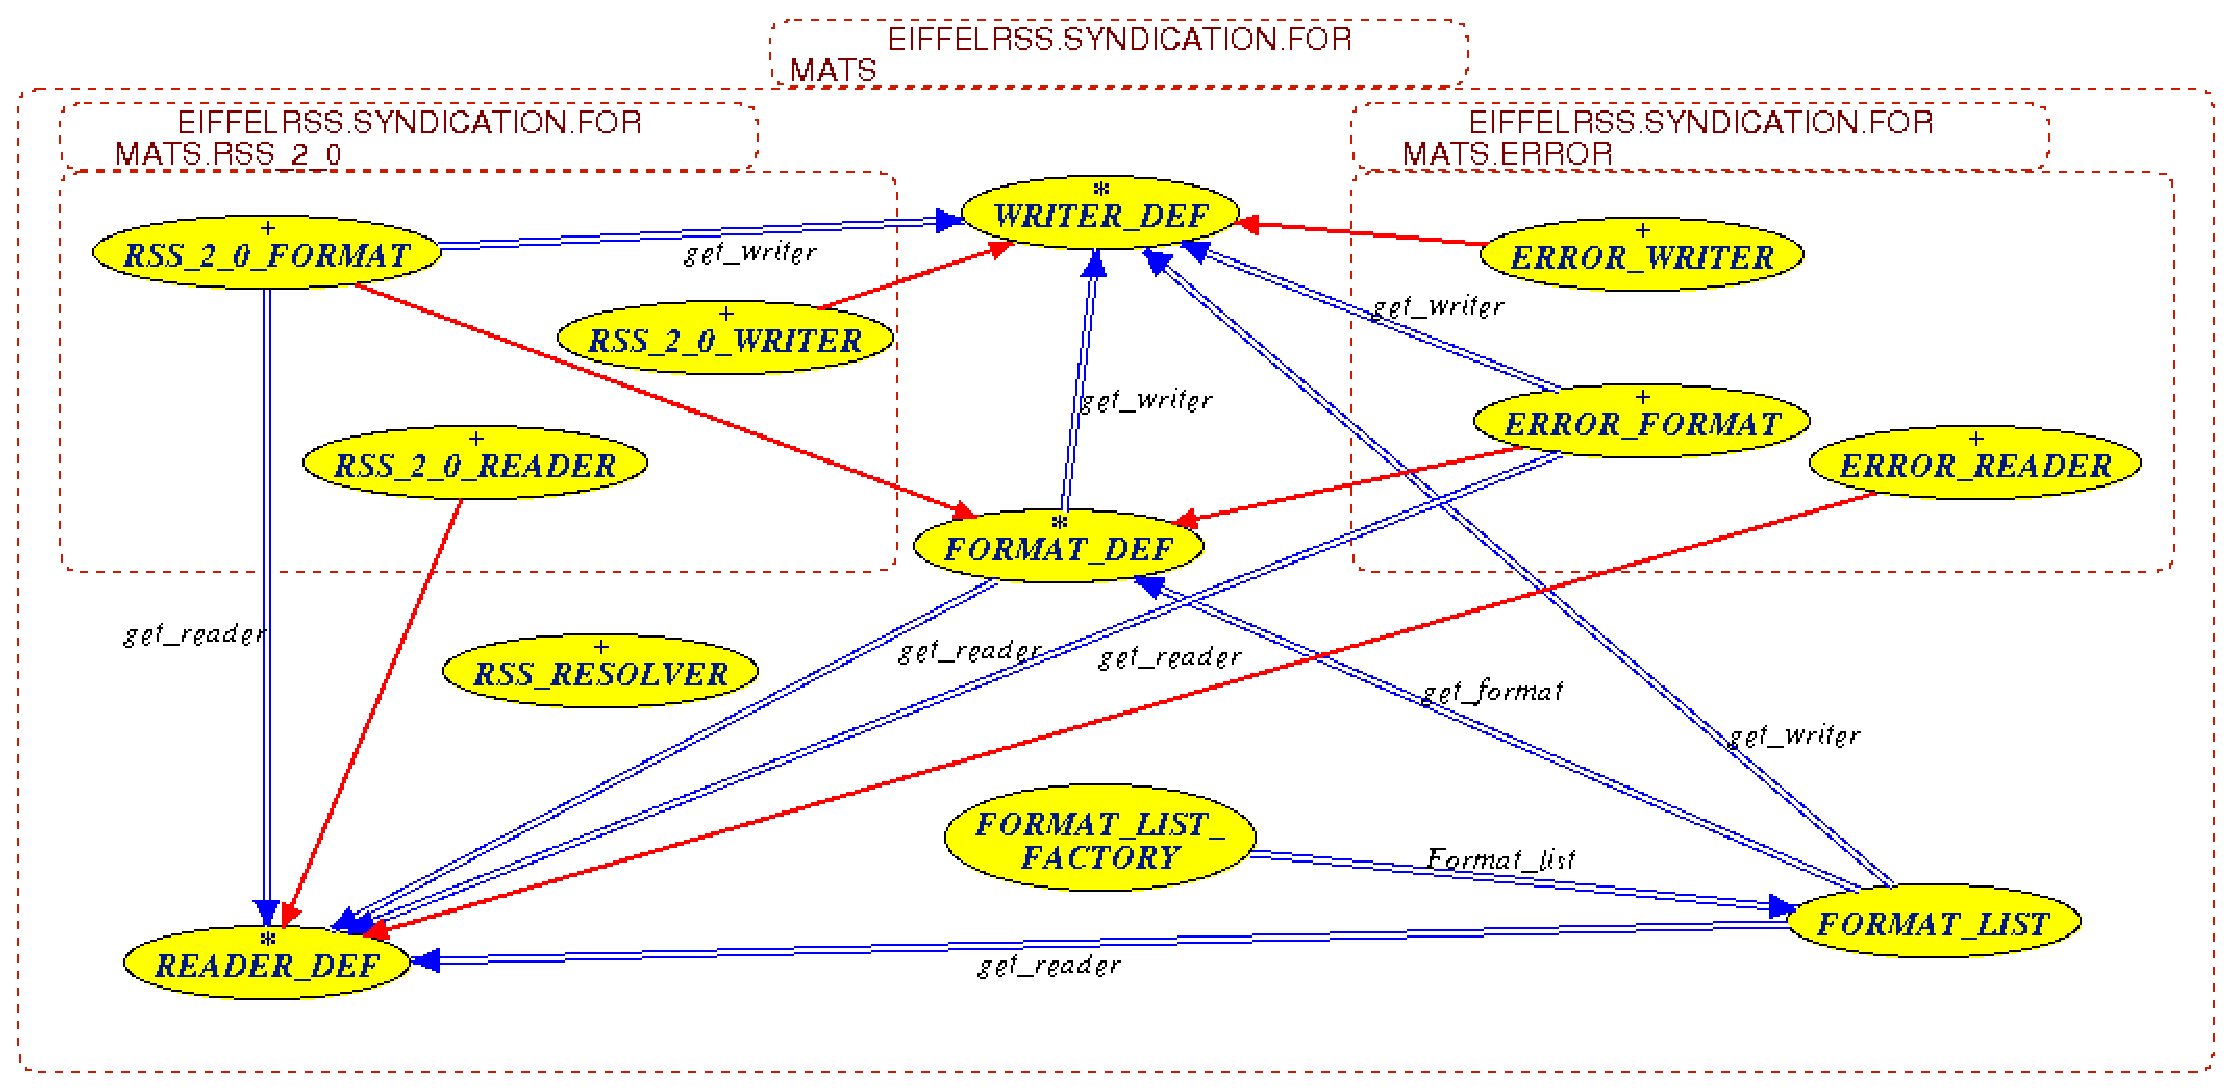
\includegraphics[width=\textwidth]{./figures/EIFFELRSS_SYNDICATION_FORMATS}
  \caption{BON diagram of cluster \texttt{FORMATS}}
  \label{fig:formats}
\end{figure}


\chapter{Management: Class FORMAT\_LIST}
\label{cha:management}


\section{Overview}
\label{sec:management-overview}

\texttt{FORMAT\_LIST} manages the different formats.


\section{Usage}
\label{management-usage}

\texttt{FORMAT\_LIST} uses a singleton pattern, so to actually use the
format list your class has to inherit from
\texttt{FORMAT\_LIST\_FACTORY}.

\texttt{FORMAT\_LIST} inherits from \texttt{LINKED\_LIST}, so all the
features of \texttt{LINKED\_LIST} are availabe as well.


\section{Features}
\label{sec:management-features}


\subsection{Initialization}
\label{sec:management-initialization}

\subsubsection{make\_list}

\begin{lstlisting}[language=Eiffel]
make_list
  -- Create the object and add the default formats
\end{lstlisting}


\subsection{Access}
\label{sec:management-access}

\subsubsection{get\_reader}

\begin{lstlisting}[language=Eiffel]
get_reader (a_name: STRING): READER_DEF
  -- Get the reader object for the name `a_name'
\end{lstlisting}

\subsubsection{get\_writer}

\begin{lstlisting}[language=Eiffel]
get_writer (a_name: STRING): WRITER_DEF
  -- Get the writer object for the name `a_name'
\end{lstlisting}

\subsubsection{get\_format}

\begin{lstlisting}[language=Eiffel]
get_format (a_name: STRING): FORMAT_DEF
  -- Get the format object for the name `a_name'
\end{lstlisting}


\subsection{Detection}
\label{sec:management-detection}

\subsubsection{detect\_format}

\begin{lstlisting}[language=Eiffel]
detect_format (a_document: XM_DOCUMENT): STRING
  -- Get the format name for `a_document'
\end{lstlisting}


\chapter{Format implementations}
\label{cha:formats-implementations}


\section{Addding a new format}
\label{sec:formats-new-format}

Adding a new format to EiffelRSS? is very easy. You have to provide
three objects which inherit from the deferred base classes
\texttt{FORMAT\_DEF}, \texttt{READER\_DEF} and \texttt{WRITER\_DEF}.
If you only want to implement a reader or a writer, you can return
\texttt{ERROR\_WRITER} respectively \texttt{ERROR\_READER} for the
other feature.

To actually add the format to the library, you have to extend
\texttt{FORMAT\_LIST} with an object of the format class.


\section{Base classes}
\label{sec:formats-base-classes}


\subsection{FORMAT\_DEF}
\label{sec:formats-format-def}

\subsubsection{get\_reader}

\begin{lstlisting}[language=Eiffel]
get_reader: READER_DEF
  -- Return a reader object
deferred
\end{lstlisting}

\subsubsection{get\_writer}

\begin{lstlisting}[language=Eiffel]
get_writer: WRITER_DEF
  -- Return a writer object
deferred
\end{lstlisting}

\subsubsection{get\_name}

\begin{lstlisting}[language=Eiffel]
get_name: STRING
  -- Return the format name
deferred
\end{lstlisting}

\subsubsection{is\_of\_format}

\begin{lstlisting}[language=Eiffel]
is_of_format (a_document: XM_DOCUMENT): BOOLEAN
  -- Is this document a feed of our type?
\end{lstlisting}


\subsection{READER\_DEF}
\label{sec:formats-reader-def}

\subsubsection{read}

\begin{lstlisting}[language=Eiffel]
read (a_document: XM_DOCUMENT): FEED
  -- Parse the document and return a feed
deferred
\end{lstlisting}

\subsubsection{get\_name}

\begin{lstlisting}[language=Eiffel]
get_name: STRING
  -- Return a string with the format name
deferred
\end{lstlisting}

\subsubsection{read\_or\_default\_element}

\begin{lstlisting}[language=Eiffel]
read_or_default_element (a_element: XM_ELEMENT; default_value: STRING): STRING
  -- Read the text of `a_element' or use `default_value' if `a_element' is Void or empty
\end{lstlisting}

\subsubsection{read\_or\_default\_attribute}

\begin{lstlisting}[language=Eiffel]
read_or_default_attribute (a_attribute: XM_ATTRIBUTE; default_value: STRING): STRING
  -- Read the value of `a_attribute' or use `default_value' if `a_element' is Void or empty
\end{lstlisting}

\subsubsection{valid\_element\_text}

\begin{lstlisting}[language=Eiffel]
valid_element_text (an_element: XM_ELEMENT; a_name: STRING): BOOLEAN
  -- Has the subelement `a_name' of `an_element' text?
\end{lstlisting}

\subsubsection{read\_date}

\begin{lstlisting}[language=Eiffel]
read_date (a_string: STRING): DATE_TIME
  -- Convert an RFC 822 date string to a DATE_TIME object
\end{lstlisting}


\subsection{WRITER\_DEF}
\label{sec:formats-writer-def}

\subsubsection{get\_name}

\begin{lstlisting}[language=Eiffel]
get_name: STRING
  -- Return a string with the format name
deferred
\end{lstlisting}

\subsubsection{writer}

\begin{lstlisting}[language=Eiffel]
write (a_feed: FEED): XM_DOCUMENT
  -- Export `a_feed' into an xml document
deferred
\end{lstlisting}


\section{Built-in formats}
\label{sec:formats-built-in}


\subsection{RSS 2.0}
\label{sec:formats-rss2}

\texttt{RSS\_2\_0\_FORMAT} is an example implementation of the RSS 2.0
standard. It reads almost all the possible data and has a very basic
writer.


\subsection{Error}
\label{sec:formats-error}

\texttt{ERROR\_FORMAT} is a special format which is used whenever an
error occurs. This removes a lot of sources of errors because the
library can ensure that the reader and writer objects are never
\texttt{Void}.

\texttt{ERROR\_READER} returns a generated feed which has one item
with the error message as description.

\end{document}
